\section{Fehlereingrenzung}
\label{sec:error-refinement}
Das Ergebnis einer Verifikation, die die Kontrakt-Spezifikationen zur Optimierung verwendet, sind eine oder mehrere Fehlerspuren.
Diese geben eine zeitlich geordnete Kette von Bedingungen über die Variablen der Komponenten des Systems.
Ein Beispiel für eine solche Spur ist die Kette
\[ \left[ (a<3,b\in \{3,5,6\}), (a > 4), (b\neq 5) \right] \]
Diese Kette von Bedingungen spezifiziert aber nicht ein Verhalten, sondern mehrere.
Die folgenden Verhalten des Systems sind beispielsweise spezifiziert:
\[ \left[ (a=2,b=3), (a=6), (b = 1) \right] \]
\[ \left[ (a=1,b=3), (a=5), (b = 1) \right] \]
Aus dieser Menge von spezifizierten Verhaltensweisen müssen nun nicht alle einen echten Fehler des Systems darstellen.
Tatsächlich reicht es, wenn ein Verhalten einen Fehler hervorruft.
Möglich ist aber auch, dass die Kontrakte dem System ein Verhalten erlauben, was das echte System niemals erzeugt.
In diesem Fall ist die Spezifikation des Systems zu grob und die Fehlerspuren nicht immer echte Fehler.

Um nun herauszufinden, welche konkreten Fehlerspuren das spezifizierte System nun tatsächlich hat, wird eine erneute Verifikation durchgeführt.
Diesmal wird das echte Systemverhalten als Grundlage herangezogen, wobei aber das Verhalten auf die Spuren begrenzt wird, die durch die Fehlerspur angegeben werden.
Meldet die Verifikation des so eingegrenzten Systems ebenfalls einen Fehler, so erhält man nicht nur die Bestätigung, dass die vorher erzeugte Fehlerspur echt ist, sondern auch ein konkretes Systemverhalten, dass zu einem Fehler führt.
Zeigt sich kein Fehler, so kann dies ein Hinweis sein, dass nicht genügend scharfe Kontrakte formuliert wurden.

\begin{figure}[h]
  \centering
  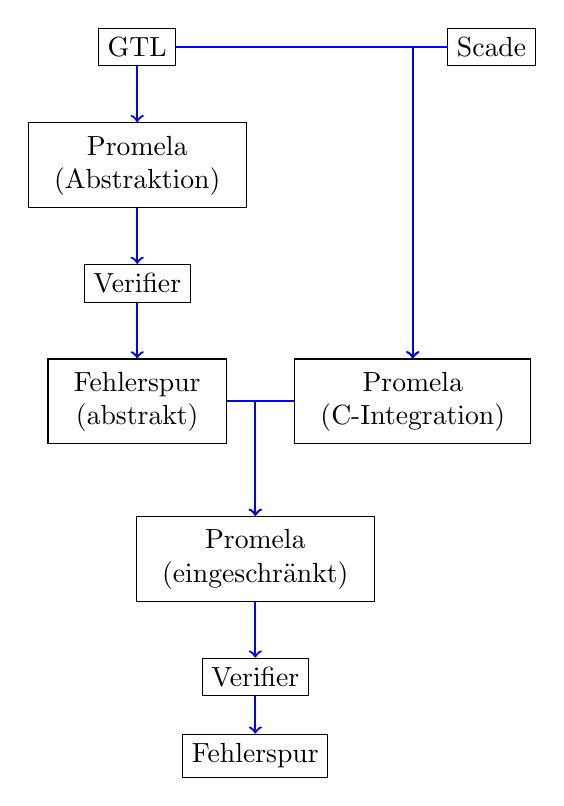
\begin{tikzpicture}
    \node[draw] (gtl) at (0,10) {GTL};
    \node[draw] (scade) at (4.5,10) {Scade};
    \node[draw] (pr1) at (0,8.5) {\begin{tabular}{c}Promela\\(Abstraktion)\end{tabular}};
    \node[draw] (ver1) at (0,7) {Verifier};
    \node[draw] (trace1) at (0,5.5) {\begin{tabular}{c}Fehlerspur\\(abstrakt)\end{tabular}};
    \node[draw] (pr2) at (3.5,5.5) {\begin{tabular}{c}Promela\\(C-Integration)\end{tabular}};
    \node[draw] (pr3) at (1.5,3.5) {\begin{tabular}{c}Promela\\(eingeschränkt)\end{tabular}};
    \node[draw] (ver2) at (1.5,2) {Verifier};
    \node[draw] (trace2) at (1.5,1) {Fehlerspur};
    \draw[->,blue,thick] (gtl) -- (pr1);
    \draw[->,blue,thick] (pr1) -- (ver1);
    \draw[->,blue,thick] (ver1) -- (trace1);
    \draw[->,blue,thick] (trace1) -| (pr3);
    \draw[->,blue,thick] (pr2) -| (pr3);
    \draw[->,blue,thick] (gtl) -| (pr2);
    \draw[->,blue,thick] (scade) -| (pr2);
    \draw[->,blue,thick] (pr3) -- (ver2);
    \draw[->,blue,thick] (ver2) -- (trace2);
  \end{tikzpicture}
  \caption{Fehlereingrenzung}
  \label{fig:error-refinement}
\end{figure}

Um diese Technik konkret umsetzen zu können, müssen an vielen Stellen der Implementierung Erweiterungen vorgenommen werden.
Hierzu betrachten wir Abbildung \ref{fig:error-refinement}:
\begin{itemize}
\item Zunächst muss der aus der GTL-Spezifikation generierte Promela-Code in der Lage sein, Fehlerspuren zu erzeugen, die Aufschluss darüber geben, welche Transitionen des generierten Büchi-Automaten zu dem Fehler führten.
  Zwar erzeugt auch SPIN schon Fehlerspuren, jedoch geben diese Auskunft über die Ausführungsposition im Quelltext und sind daher extrem schwer zurück auf die Zustände des Büchi-Automaten zu rechnen.
  Die hier verwendete Lösung besteht darin, im generierten Quelltext vor jedem Betreten eines Zustands mit der \emph{printf}-Anweisung eine Ausgabe zu erzeugen, die den Namen des betretenden Zustands enthält.
  Spielt man eine generierte Fehlerspur nun in SPIN ab, so erhält man genau die Ausgaben für die betretenden Zustände und kann eine genaue Fehlerspur für den Büchi-Automaten berechnen.
\item Die Fehlerspur wird kodiert als eine Liste, in der jedes Element einem Zeitschritt entspricht.
  Ein Element enthält eine Abbildung von den Variablen des Systems auf BDDs, die den erlaubten Wertebereich dieser Variablen zum Zeitpunkt des Elements festlegen.
\item Die so generierte Fehlerspur muss jetzt noch benutzt werden, um in der Verifikation per C-Integration die Pfade zu beschränken.
  Dies geschieht, indem die Schnittmenge des generierte Büchi-Automat für die zu verifizierende Eigenschaft und des Automaten aus der Fehlerspur gebildet wird.
  Damit werden im Modell nur Pfade verifiziert, die der Fehlerspur entsprechen.
\end{itemize}
